\documentclass[10pt]{article}

\def\Type{LessonCaelan}
\def\TypeNum{Lesson 18}
\def\TypeTitle{Fundamental Theorem of Calculus }
\def\Semester{Fall 2021} %Not Used 
\def\Course{MATH 1190 \& 1210}
\def\Targets{  \bf\color{Fuchsia}I3, \bf\color{Fuchsia}I4 }

\usepackage{preambleDJ}

%\usepackage{ragged2e}


%%%%%%%%%%%% BEGIN DOCUMENT %%%%%%%%%%%%%%%
%%%%%%%%%%%% BEGIN DOCUMENT %%%%%%%%%%%%%%%
%%%%%%%%%%%% BEGIN DOCUMENT %%%%%%%%%%%%%%%
%%%%%%%%%%%% BEGIN DOCUMENT %%%%%%%%%%%%%%%
%%%%%%%%%%%% BEGIN DOCUMENT %%%%%%%%%%%%%%%




\begin{document}

\pagestyle{otherpages}
\thispagestyle{firstpage}
\vs{.5}

\textbf{Intended Learning Outcomes}
After this lesson, you will be able to 

\begin{itemize}
    \item Use the Fundamental Theorem of Calculus to evaluate a definite integral. (\target{I4})
    \item Identify when the Fundamental Theorem of Calculus does not apply. (\target{I4})
\end{itemize}

\vspace{-0.6cm}

\hrulefill\\

{\bf\color{blue}Warm-up Exercise 1.}\ltrm{\bf\color{Fuchsia}I3} Find in the following indefinite integrals.
\def\vd{.3}
\tasksA{2}{
\task $\dint e^x \,dx=$
\task $\dint 3^x \,dx=$ \vs{\vd}
\task  $\dint \frac{1}{x^2} \,dx =$ 
\task $\dint \frac{1}{x} \,dx =$ \vs{\vd}
\task $\dint 2^5 \,dx =$ 
\task $\dint \log(2) \,dx =$ \vs{\vd}
\task $\dint \frac23x^4 \,dx =$
\task $\dint \sqrt{x^3} \,dx =$ \vs{\vd}
}
\blue{\bf Mini-lecture:  The Fundamental Theorem of Calculus and its hypotheses}

%maybe start off with several simple ones - like 4x^3, 1/x, etc. - and then build up to larger ones - sums of these kinds of functions - then incorporate simplification

\begin{minipage}[t]{0.6\textwidth}
    \important{Fundamental Theorem of Calculus (FTC)}
    {
    If $f$ is continuous on $[a,b]$, then
    \vspace{-.1in}
    
    \[
    \int_a^b f(x)\ dx = F(x)\bigg|_{a}^{b}
    \]
    
      where $F$ is any antiderivative of $f$ and\\ $F(x)\bigg|_{a}^{b} = \Delta F = F(b)-F(a)$.
    }
\end{minipage}
%
\hfill
%
\begin{minipage}[t]{0.375\textwidth}
\,\\[-0.4in]
    \begin{center}
        \begin{tikzpicture}[scale=0.95]
          \begin{axis}[
        %    axis y line = left,
        %    axis x line = bottom,
        x label style={anchor=west},
            xlabel = {$x$},
            y label style={anchor=south},
            ylabel={$y$},
            %xtick       = {0.5,4.45},
            %xticklabels = { , },
            ytick       = {2.5,4.5,6.5,8.5},
            yticklabels = {$2$,$4$,$6$,$8$},
            samples     = 160,
            domain      = -2.5:2.5,
            restrict y to domain=-0.5:9.5,
            xmin = -2.5, xmax = 2.5,
            ymin = -0.5, ymax = 9.5,
            width = 3in, height=2in
          ]
          % piece 1
          \addplot[domain=-2.5:0.01, blue, ultra thick, <->] {1/x^2+.5};
          % piece 2
          \addplot[domain=0.01:2.5, blue, ultra thick, <->] {1/x^2+.5};
          \node at (1.5,6) {$f(x)=\dfrac1{x^2}$};
          \end{axis}
        \end{tikzpicture}
    \end{center}
\end{minipage}\\
%
\blue{\bf Example/Exercise}\ltrm{\bf\color{Fuchsia}I4} For each of the definite integrals below, a) Decide if $\ds \int_a^b \frac{1}{x^2}\,dx$ should be positive or negative. b) Calculate each definite integral. c) Discuss if your answer to a) and b) are consistent. \vs{-.1}\\
\mpageT{.49}{.49}[\vline]{
  \enumA{
  \item Based on graph, should $\dint_{1}^{2} \frac{1}{x^2}\,dx$ be positive or negative?\vs{.1}
  \item  $\dint_{1}^{2} \frac{1}{x^2}\,dx=$\vs{.75}
  \item Is your answer to a) consistent with b)? If not, what about the FTC might help us understand why not?\vs{.5}
}
}{
%
%\vline\hfill
%
  \enumA{
  \item Based on graph, should $\dint_{-2}^{1} \frac{1}{x^2}\,dx$ be positive or negative?\vs{.1}
  \item $\dint_{-2}^{1} \frac{1}{x^2}\,dx=$\vs{.75}
  \item Is your answer to a) consistent with b)? If not, what about the FTC might help us understand why not?\vs{.5}
}
}

\vspace{3cm}

%\newpage


\exercise\ltrm{\bf\color{Fuchsia}I4}   For each of the following definite integrals, decide if the Fundamental Theorem applies.  If it does, evaluate the integral.\\

\tasksA{2}{
\task $\displaystyle\int_0^2 2x \,dx$ \qquad FTC apply?
\task $\displaystyle\int_{-2}^{-1} \sqrt{x} \,dx$ \qquad FTC apply?
}
\vs{.2}
\tasksI{2}{
\task If ``yes", \\$\displaystyle\int_0^2 2x \,dx$=
\task If ``yes"\\$\displaystyle\int_{-2}^{-1} \sqrt{x} \,dx=$
}
\vs{1}



\ltrm{\bf\color{Fuchsia}I4}  \example Evaluate the following integrals: {\em Hint:} It might be helpful to a bit of algebra first so that you can use one of our derivative rules.

\begin{itemize}

\item[(a)] $\dint_1^2 \left( \dfrac{2}{\sqrt[5]{t^3}} + 3^t - \frac12 \right)\,dt$
    
    \vfill

\item[(b)] $\dint_2^4 \dfrac{z^2-z-1}{2z}\,dz$

    \vfill

\end{itemize}
\newpage
\exercise \ltrm{\bf\color{Fuchsia}I4}  Evaluate the following integrals:

\begin{itemize}

\item[(a)] $\dint_{-2}^{-1} \left( \dfrac{4}{\sqrt[3]{u}} + e^u + 2u^3 \right) \, du$

\vs{1.75}

\item[(b)] $\displaystyle\int_{1}^2 \frac{1+\sqrt[4]{y}+\sqrt{y}+y}{y} \, dy$

  \vs{1.75}

\end{itemize}



{\bf\color{blue}Extra Practice 1.} Evaluate the following integrals:

\begin{itemize}

\item[(a)] \ltrm{\bf\color{Fuchsia}I3}  $\dint \left(x^2+x+1\right)\,dx$ \\
\vs{.5}
\item[(b)] \ltrm{\bf\color{Fuchsia}I4}  $\dint_0^1 \left(x^2+x+1\right)\,dx$

\vs{.75}
\item[(c)] \ltrm{\bf\color{Fuchsia}I4}  $\dint_{1/8}^1 \left( \dfrac{x^2+x+1}{\sqrt[3]{x}} \right)\,dx$

\vs{1.25}

\end{itemize}
\newpage
{\bf\color{blue}Extra Practice 2.} \ltrm{\bf\color{Fuchsia}I4}  The graph of $f(x)=x^3$ is given below.\\

\mpageT{.35}{.65}{    
\begin{center}
        \begin{tikzpicture}
          \begin{axis}[
            xmin=-2.5,        % Minimum x-value
            xmax=2.5,         % Maximum x-value
            ymin=-8,         % Minimum y-value
            ymax=8,          % Maximum y-value
            axis lines=middle, % Draw the x and y axes in the middle
            xlabel={$x$},     % Label for the x-axis
            ylabel={$y$},     % Label for the y-axis
            xtick       = {-2,-1,1,2},
            ytick       = {-8,-4,4,8},
            %yticklabels = {$2$,$4$,$6$,$8$},
            axis line style={thick, <->}, % Add arrows at the end of the axes
            width = 2in, height=2in,
            %restrict y to domain=-6.5:6.5
          ]
          %\addplot[domain=-2.5:2.5, samples=400, blue, ultra thick] {x^3};
              \addplot[name path=f1, domain=-2.5:2.5, blue, ultra thick, <->] {x^3};
%  \path[name path=axis] (axis cs:-2.5,0) -- (axis cs:2.5,0);
%     \addplot [
%        thick,
%        color=blue,
%        fill=blue, 
%        fill opacity=0.1
%    ]
%    fill between[
%        of=f1 and axis,
%        soft clip={domain=-1:2},
%   ];
          \end{axis}
        \end{tikzpicture}
    \end{center}
}{
%
\begin{itemize}
\item[(a)] Find the {\bf net area} between the graph of $f(x) = x^3$ and the portion of the horizontal axis from $x=-1$ to $x=2$.
\end{itemize}
}
\vs{.5}
\begin{itemize}
\item[(b)] Find the {\bf area} between the graph of $f(x)=x^3$ and the portion of the horizontal axis from $x=-1$ to $x=2$.

\end{itemize}


\end{document}\end{document}
